\documentclass{article}
\usepackage{pgfplots}
\pgfplotsset{compat=1.16}

\begin{document}

\begin{figure}[h]
    \centering
    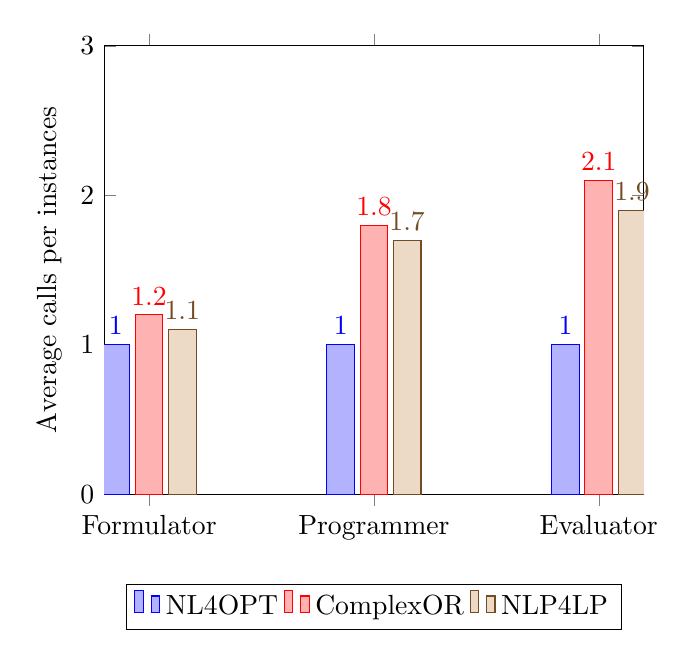
\begin{tikzpicture}
        \begin{axis}[
            ybar,
            ylabel={Average calls per instances},
            symbolic x coords={Formulator, Programmer, Evaluator},
            xtick=data,
            ymin=0,
            ymax=3,
            legend style={at={(0.5,-0.2)}, anchor=north,legend columns=-1},
            nodes near coords,
            nodes near coords align={vertical},
            ]
            \addplot coordinates {(Formulator, 1) (Programmer, 1) (Evaluator, 1)};
            \addplot coordinates {(Formulator, 1.2) (Programmer, 1.8) (Evaluator, 2.1)};
            \addplot coordinates {(Formulator, 1.1) (Programmer, 1.7) (Evaluator, 1.9)};
            
            \legend{NL4OPT, ComplexOR, NLP4LP}
        \end{axis}
    \end{tikzpicture}
    \caption{Average number of calls to each agent among solved problems. OptiMUS only requires one call per agent on the simple problems of NL4OPT. On the more complex datasets, it relies more heavily on the programmer to fix errors identified by the evaluator, but rarely improves by fixing formulation errors.}
    \label{fig:calls_per_agent}
\end{figure}

\end{document}